\documentclass[a4paper,10pt,twocolumn,uplatex]{jsarticle}
\usepackage{style/nislab,style/resume}

%---------------------------------------------------------------------
% レジュメ種別・日付設定(要変更)
% \type{} 1:修士論文諮問会 2:卒業論文発表会 3:月例発表会 4:研究室合同発表会
%---------------------------------------------------------------------
\type{3}
\year{2022}
\month{6}
\date{11}

%---------------------------------------------------------------------
% ページ番号設定(要変更)
%---------------------------------------------------------------------
\setcounter{page}{1}

%---------------------------------------------------------------------
% 変更不要
%---------------------------------------------------------------------
\begin{document}

%---------------------------------------------------------------------
% タイトル作成部分(要変更)
% \maketitle{タイトル}{title}{名前}{name}
%---------------------------------------------------------------------
\maketitle{タイトルタイトルタイトルタイトルタイトルタイトル}
{Title Title Title Title Title Title}
{竹内 一真}
{Kazuma Takeuchi}

% --------------------------- Section1  ---------------------------

\section{はじめに}
近年,多方面でのドローンを活用した事業が進出しており,インフラ点検や災害調査など,応用分野を拡大しながら,世界のドローン市場は急速に成長している\cite{Nonami}.
中でも小型ドローンの特徴である機体の大きさを活かして,人間が入れないような狭い空間での活躍の場も増加している.
しかし,狭小空間でのドローン飛行は,遮蔽物が多く,操縦者は遮られた視点からの操縦を必要とする.
そのため,死角領域内のドローン操縦では,ドローンを視認できない中,衝突することなく,安全に操縦する技術が求められる.
\par
オンボードカメラ搭載ドローンを使用する場合では,操縦者は,ドローンから送られる空撮した映像を元に操縦が可能となる.
このようなドローン操縦方法では,実際の現実空間を映像として見ながら操縦できるため,現実のドローンを視認することなく,狭小空間を探索することができる.
しかし,カメラが前方しか写さないことにより,前方以外の死角が多くなり,状況認識が不十分となるため\cite{Green},狭小空間のように狭く,障害物が多いような環境では,操縦は困難である.
大型ドローンでは,自律飛行や障害物回避などの機能が実現されているが,センサ搭載制限のある小型ドローンでは,障害物回避の支援がないことが多く,衝突の危険性があり,
また,障害物回避の機能を搭載していても,狭小空間では障害物回避が行えない場面が多く存在する\cite{syohou}.
\par
そこで,Augmented Reality(AR)を用いて死角領域内を可視化することで,ドローンの操縦性向上や安全性向上が期待されている.
事前に走行環境をマッピングすることで3次元環境地図を取得し,空間認識を提供している.
しかし,狭小空間のドローン操縦において,事前に3次元環境地図を用意することは困難なため,
走行環境を探索する中で,リアルタイムにマッピングを行う必要がある.また,複数ドローンが混在する場合も問題である.
各ドローンがマッピングした3次元環境地図が異なるため,精度が悪く,操縦者の空間認識に悪影響を及ぼすため,作成した3次元環境地図を
統一し,精度を向上する必要がある.
% 操縦者視点でドローンを視認し飛行させる三人称視点操縦の場合では,ドローン中心の一人称視点での操縦に比べて,ドローン周辺の状況を把握することができ,また,ドローンの実際の高さや位置を正確に把握することができる\cite{Green}.
% しかし,三人称視点操縦では,操縦者から見えるドローンまでの距離感が掴めないため\cite{Zollmann},ドローン周辺の障害物へ衝突する恐れがある.
% 大型ドローンでは,自律飛行や障害物回避などの機能が実現されているが,センサ搭載制限のある小型ドローンでは,障害物回避の支援がないことが多く,衝突の危険性がある.
% また,障害物回避を搭載していても,狭小空間では障害物回避が行えない場面が多く存在する\cite{syohou}.
本研究では,狭小空間による死角領域内の複数ドローン飛行の危険性を軽減するため,ARにより操縦者の死角領域内を可視化し,リアルタイムに3次元環境地図を作成し,合成するシステムを開発する.

% --------------------------- Figure  ---------------------------

% \begin{figure}[!tb]
%   \centering
%   
\includegraphics[width=\linewidth]{img/sample1.pdf}
%   \caption{悩む男の子}
%   \label{fig:sample1}
% \end{figure}

% \begin{figure*}[!tb]
%   \centering
%   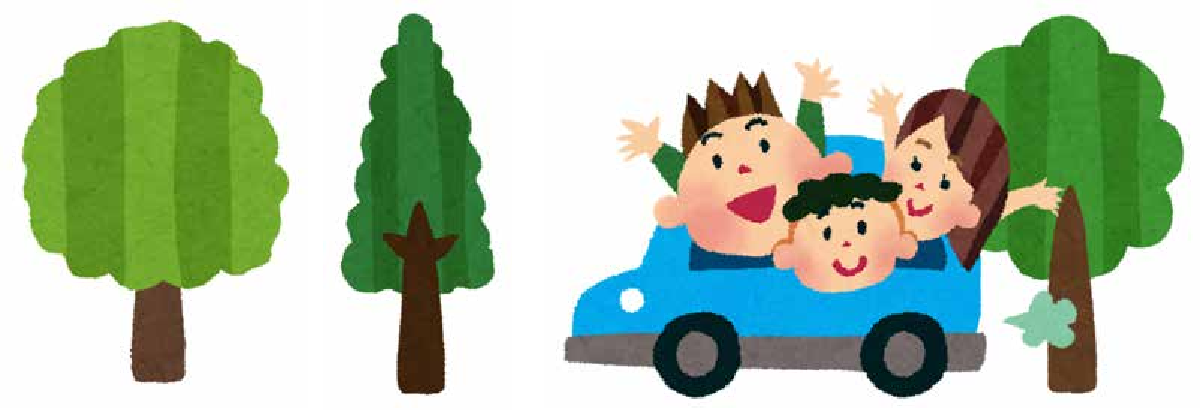
\includegraphics[width=\linewidth]{img/sample2.pdf}
%   \caption{ドライブする家族}
%   \label{fig:sample2}
% \end{figure*}

% --------------------------- Section2  ---------------------------

\section{提案システム}
\subsection{概要}
本研究では,狭小空間により,操縦者と小型ドローン(以下,ドローン)の間に遮蔽物があり,ドローンを視認できない環境を「死角領域」とする.
図\ref{fig:03_enviroment}の環境におけるドローン操縦を想定しており,ARを用いて死角領域内の空間認識を提供し,ドローン周辺の障害物を知覚させることで,ドローン操縦性を向上させる.
\par
先に述べた先行研究\cite{Erat}を元に,2つのドローン操縦方式を用意し,一人称視点方式,可視化方式と呼ぶことにする.
図\ref{fig:03_FPV}に示しているようなドローンの空撮した映像を頼りに操縦を行う,従来のドローン操縦手法である一人称視点方式と,
\ref{fig:02_relation}を参考に作成した,ARを用いて死角領域内の空間認識を提供する可視化方式を比較することにより,先行研究の問題点である,死角領域内へのAR適用の有用性を検討する.
また,本研究では可視化方式を元に,ドローン周辺の障害物知覚を支援する2つの方式を提案する.
この2つの方式を,距離画像方式,マーカー方式と呼ぶことにする.
4つの方式を比較することで,どのような情報が死角領域内のドローン操縦に有効であり,操縦性の向上を示せるか評価した.
各方式の概要を図\ref{fig:03_outline}に示す.以降の節では一人称視点方式,可視化方式,距離画像方式,マーカー方式の4つの方式の詳細について説明する.

\subsection{死角領域内のAR可視化}

\subsection{3次元環境地図の生成}
自己位置推定

データの収集

点群データのポリゴン化
センサーデータの重ね合わせによって生成した3次元地図は、膨大な数の点の集合 であり、データ量が非常に大きく扱いづらい。
そこで建物の内装を構成する主な要素である壁や床といった 平面に着目し、点群データから平面を抽出しポリゴン化することで、
3次元地図のデータ量を大幅に削減する 仕組みを実現した。
% --------------------------- Section3  ---------------------------

\section{評価}

\subsection{実装環境}
システム構成を図\ref{fig:04_system}に示す.
使用するドローンはRyze Tech社製Tello EDU(以下,Tello)を用いる.Telloはプログラミングによってフライトコントロールを行うことができ,
規定のコマンドを送信することで飛行制御することができる.
\par
ARHMDはMicrosoft HoloLens2(以下,HoloLens)を使用する.
システムはHoloLens2上でUnityアプリケーションが動作しており,Unity内で仮想ドローン,3次元環境地図を配置する.
サーバでは常時Telloの位置情報をHoloLens2に送信する.
受け取った値をUnity座標系へ変換し,変換後の値を反映させることにより,仮想的に死角領域内を可視化している.
\par
サーバではTello,HoloLensとUDP通信を行なっており,常時,Telloの傾きや移動距離をHoloLensに送信することで,3D仮想空間上に存在するドローンとの位置合わせを行っている.
ここでUDPを使用する理由として,Tello,サーバ,HoloLens間の遅延低減を目的とする.
\par
距離画像方式,マーカー方式では,共に障害物までの距離によって,危険度を色で示している.操縦者がドローンを操縦するとき,衝突する危険性がある距離を0.3mとし\cite{Yamada},
距離画像方式では,障害物までの距離が0.3mまでを赤色,0.3m〜0.6mまでを黄色,0.6m以上を緑色で示す.マーカー方式では障害物までの距離が0.3mまでを赤色の目印,
0.3m〜0.6mの際に黄色の目印を示す.

% --------------------------- Figure  ---------------------------

% \begin{figure}[tb]
%   \centering
%   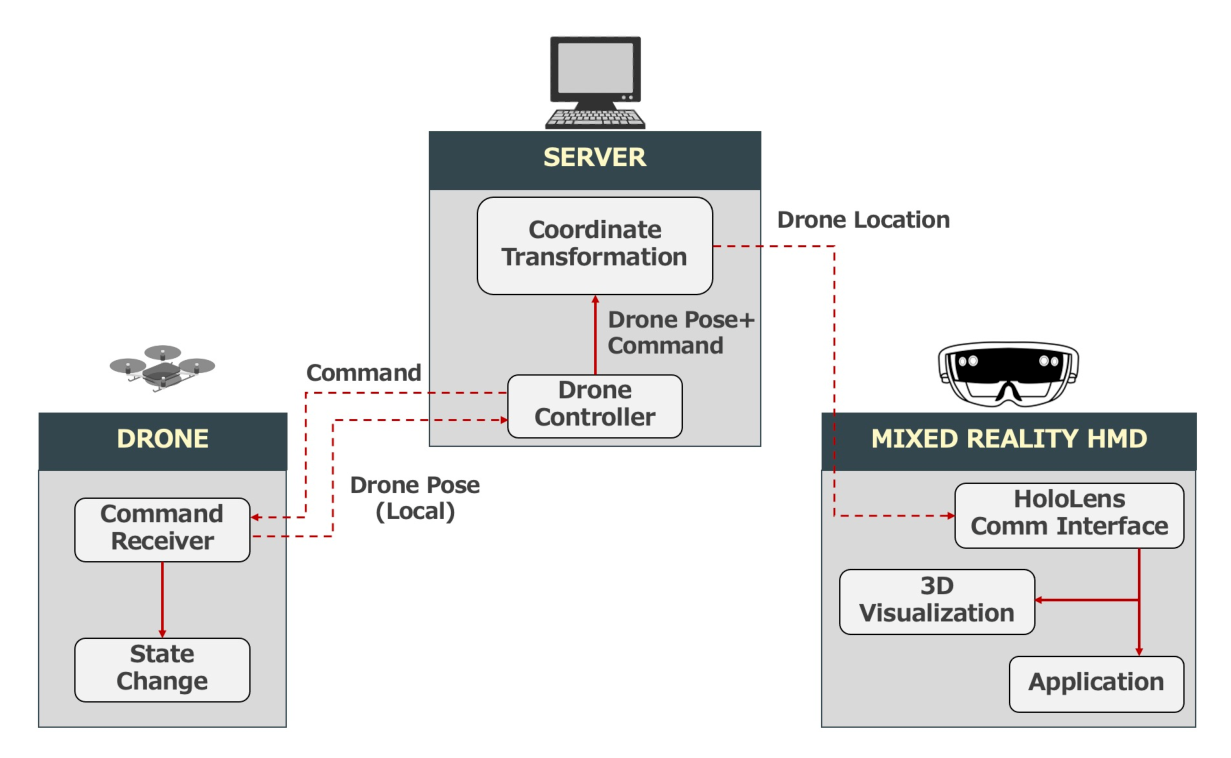
\includegraphics[width=\linewidth]{img/04_system.eps}
%   \caption{システム構成}
%   \ecaption{System Configuration}
%   \label{fig:04_system}
%   \end{figure}
  
% -----------------------------------------------------------------

\subsection{実験}
死角領域内を飛行するドローンの操縦において,各方式がどのような影響を与えるかを評価するため,10人の実験協力者による実験を行なった.参加者の平均年齢は22歳であり,
ドローン操縦経験はなかった.
実験は約60分で行い,導入,各提案方式の練習,ARのキャリブレーション,タスク,アンケートの5つのフェーズから構成する.
まず,参加者は本研究の概要と,操縦方法の説明を受け,その後,各方式の練習を行う.予備実験で,操縦の慣れによる実験後半の操縦時間短縮や,
ARの経験がないことによる操縦時間増加を引き起こすことがわかった.そのため,この効果を打ち消すために,ドローン操縦を5〜10分ほど練習した後に,
各方式で実験環境を1度走行することで,練習量を増やし,慣れによる差異を無くした.
次にAR方式では,HoloLensアプリケーションを起動し,現実空間とのキャリブレーションを行い,参加者はHoloLensを装着した.
その後,タスクを行い,各方式でタスクを完了する度に,実験を行なった方式についてアンケートを記入し,全方式を終了したら,
どの方式が最も効果的であったかを選択し,その理由を記入してもらった.また,なぜ他の方式を選択しなかったのかの理由も記入してもらった.


\subsection{評価項目}
提案方式の有効性を評価するにあたり,ドローン技術の熟練度による差を出さないために,Telloの速度,一度に進む距離,旋回角度は事前に設定している.またサーバのスペック,サーバよりTelloへ送信するコマンドのパラメータの設定を表\ref{tab:server_spec},表\ref{tab:command_parameter}に示す.
本研究では,各方式における,操縦者がタスクを完了するまでの操縦時間,障害物への衝突警告回数の2項目による客観的な評価と,参加者へのアンケート,自由回答による主観的な評価を記録した.障害物の衝突警告回数では,実際に衝突してしまう恐れがあるため,操縦者がドローンを進行させようとしている方向に存在する障害物との距離を計測し,距離が0.3 m以内の際に操縦者へ警告がされるようになっている.表\ref{tab:command_parameter}に示すように,ドローンの進行距離を0.3 mとしているため,衝突警告距離の閾値を0.3 mとした.また参加者へのアンケートでは,主観的な認識と好みを測定するために,7ポイントのリッカート尺度のアンケートを実施した.アンケートでは一人称視点方式とARを利用した3つの各方式を比較できるように実施し,また,AR同士での比較が行えるように,ARを用いた方式のみ別途アンケートを実施した.一人称視点方式とARを用いた3つの各方式を比較するアンケートでは,安心な操縦できたか,危険な障害物を判断できたかの2項目を設けた.また,ARを用いた方式のみを比較するアンケートでは,状況把握が容易だったか,自信を持って操縦を行えたかの2項目を設けた.実験の最後には,参加者にはどの方式が最も操縦性が良かったかを選択し,なぜその方式が良かったのか,また,なぜ他の方式を選択しなかったかという項目を設けた.タスク完了までの平均操縦時間には一次元配置分散分析(one-way analysis of variance:以下,ANOVA)を用いて統計解析した.また,Post-hoc検定では,Tukey’s Honestly Significant Difference(Tukey HSD)検定を行い,各方式の比較を行なった.平均衝突警告回数,アンケート結果では,Friedman検定を行い,Post-hoc検定ではBonferroni法を行い,各方式の比較を行なった.

% -----------------------------------------------------------------

% --------------------------- Section4  ---------------------------

\section{おわりに}

小型ドローンは機体の大きさを活かして,インフラ点検や災害調査のような,人間が立ち入れない狭小空間での活躍が増えている.しかし,狭小空間でのドローン飛行では,遮蔽物による視点が遮られる死角領域内での操縦を必要とする.また,従来の操縦法では状況認識が不十分であるため,ドローン周辺に位置する障害物が多い狭小空間では,ドローン操縦は困難である.\par
遮蔽物,障害物が多い狭小空間では,死角領域内におけるドローン飛行の危険性を軽減する必要がある.
そこで本研究では,ARにより操縦者の死角領域内に存在するドローンと周辺環境を可視化し,ドローン周辺の障害物を知覚するためのAR方式を提案する.
本提案方式について,死角領域内でのドローン操縦性を評価実験した.
結果として,ARを利用した方式では実験環境での操縦時間が短く,衝突回数も少なかったことから,狭小空間による死角領域内のドローン操縦性向上を示した.
また,障害物を知覚するためのAR方式では,ドローン周辺の障害物に対し,危険度を色で振り分けている方式が操縦者へ安心を与え,操縦性を向上させたことを示した.

%---------------------------------------------------------------------
% Bibliography(参考文献)
%---------------------------------------------------------------------
% thebibliography を利用する場合は以下を使用
\footnotesize{
  \begin{thebibliography}{99}
    \bibitem{LaTexWiki} Latex Wiki. \url{https://texwiki.texjp.org/}.
    \bibitem{渡辺豊2016} 渡辺 豊, "角皆静男先生のご逝去を悼む", 地球化学, vol.50, no.1, pp.1-3, 2016.
  \end{thebibliography}
}

% BibTex を利用する場合は以下を使用(初めての人には難しいかも)
% \bibliographystyle{junsrt}
% \bibliography{myref}

%---------------------------------------------------------------------
\end{document}
%---------------------------------------------------------------------